\documentclass[a4paper]{article}
\usepackage[utf8]{inputenc} % Skal passe til editorens indstillinger
\usepackage[english]{babel} % danske overskrifter


\newcommand{\name}{Carsten Nielsen}
%\newcommand{\stnumber}{s123369, s123161, s123821}
\newcommand{\course}{INI 404 Neuromorphic Engineering~I}
\newcommand{\university}{University of Zürich}
\newcommand{\studyline}{Institute of Neuroinformatics}
\newcommand{\assignment}{Lab 8 Post-Lab}
\renewcommand{\date}{\today} %If another date, than that of today is desiered


% Palatino for rm and math | Helvetica for ss | Courier for tt
\usepackage{mathpazo} % math & rm
\linespread{1.05}        % Palatino needs more leading (space between lines)
\usepackage{palatino} % tt
\normalfont
\usepackage[T1]{fontenc}
\usepackage[english]{babel}

\usepackage{graphicx}%allerese hentet % indsættelse af billeder
\usepackage{epstopdf} %Tilfj "--enable-write18" i argumentet for LaTex build. Dette vil konvertere .eps figurer til pdf-format
\graphicspath{{./picture/}} % stivej til bibliotek med figurer
\usepackage{subcaption} %Til gruppering af figurer
\usepackage{amsmath} %matpakke
\usepackage{amsfonts} %
\usepackage{amssymb} %
\usepackage{steinmetz} % flere matematik symboler
\usepackage{polynom} %for displaying polynom division
\usepackage{mathtools} % matematik - understøtter muligheden for at bruge \eqref{}
\usepackage{float}
\usepackage{placeins}
\usepackage{hhline}

%
\usepackage[usenames,dvipsnames]{xcolor}
\usepackage[compact,explicit]{titlesec}% http://ctan.org/pkg/titlesec
%
\usepackage[europeanresistors]{circuitikz}
\usepackage{pgfplots}
\usepgfplotslibrary{patchplots}
\pgfplotsset{compat=1.11}

%---------%
%Easy edit%
%---------%

%Section formating. arg1 is supplied when making section
\newcommand\presectionnumber[1]{~~}
\newcommand\postsectionnumber[1]{}
\newcommand\midlesection[1]{#1}
\newcommand\sectionnum[1]{\arabic{#1}}
\newcommand\subsectionnum[1]{\arabic{#1}}
\newcommand\subsubsectionnum[1]{\alph{#1}}



%------------%
%setion setup%
%------------%
\renewcommand\thesection{Opgave~\sectionnum{section}} %pas p�, kun i matematik
\renewcommand\thesubsection{\thesection,~\subsectionnum{subsection}}
\definecolor{MagRed}{RGB}{190,40,15}
\definecolor{MathGreen}{RGB}{82,164,0}

\titleformat{\section}{\normalfont\sffamily\large\bfseries\color{MathGreen}}{}{0pt}{|\kern-0.15ex|\kern-0.15ex|\kern-0.15ex|\presectionnumber{#1}\sectionnum{section}\postsectionnumber{#1}\qquad\quad\midlesection{#1}\label{sec:\sectionnum{section}}}
\titleformat{\subsection}[runin]{\large\bfseries}{}{10pt}{\sectionnum{section}.\subsectionnum{subsection})~#1\label{sec:\sectionnum{section}.\subsectionnum{subsection}}}
\titleformat{\subsubsection}[runin]{\itshape}{}{0pt}{\subsectionnum{subsection},\subsubsectionnum{subsection}~#1\label{sec:\sectionnum{section}.\subsectionnum{subsection}.\subsubsectionnum{subsubsection}}}
%\titleformat{\subsubsection}{\bfseries}{}{0pt}{\alph{subsection}.\arabic{subsubsection})\qquad\quad#1\label{\arabic{section}\alph{subsection}\arabic{subsubsection}}}

%----------%
%page setup%
%----------%
\textwidth = 400pt
\marginparwidth = 86pt
\hoffset = -25pt
\voffset= -30pt
\textheight = 670pt

%--------%
%hyperref%
%--------%
\newcommand{\HRule}{\rule{\linewidth}{0.5mm}}
\usepackage{fancyhdr}
\usepackage[plainpages=false,pdfpagelabels,pageanchor=false]{hyperref} % aktive links
\hypersetup{%
  pdfauthor={\name},
  pdftitle={\assignment},
  pdfsubject={\course} }
%\usepackage{memhfixc}% rettelser til hyperref

%-------------%
%Headder setup%
%-------------%
\fancyhf{} % tom header/footer
\fancyhfoffset{20pt}
\fancyhfoffset{20pt}
\fancyhead[OL]{\name \\ INI 404}
\fancyhead[OC]{Date \\ \date}
\fancyhead[OR]{\university\\ \studyline}
\fancyfoot[FL]{}
\fancyfoot[FC]{\thepage}
\fancyfoot[FR]{}
\renewcommand{\headrulewidth}{0.4pt}
\renewcommand{\footrulewidth}{0.4pt}
\headsep = 35pt
\pagestyle{fancy}
 % style setup

%Listings%
\usepackage{listingsutf8}
\usepackage[framed,numbered]{matlab-prettifier}


%setup listings
\lstset{language=Matlab,
  extendedchars=true,
  language=Octave,                % the language of the code
  basicstyle=\ttfamily\footnotesize,           % the size of the fonts that are
  % used for the code
  numbers=left,                   % where to put the line-numbers
  numberstyle=\tiny\color{gray},  % the style that is used for the line-numbers
  stepnumber=2,                   % the step between two line-numbers. If it's 1, each line 
                                  % will be numbered
  numbersep=5pt,                  % how far the line-numbers are from the code
  backgroundcolor=\color{white},      % choose the background color. You must add \usepackage{color}
  showspaces=false,               % show spaces adding particular underscores
  showstringspaces=false,         % underline spaces within strings
  showtabs=false,                 % show tabs within strings adding particular underscores
  frame=single,                   % adds a frame around the code
  rulecolor=\color{black},        % if not set, the frame-color may be changed on line-breaks within not-black text (e.g. comments (green here))
  tabsize=4,                      % sets default tabsize to 2 spaces
  captionpos=b,                   % sets the caption-position to bottom
  breaklines=true,                % sets automatic line breaking
  breakatwhitespace=false,        % sets if automatic breaks should only happen at whitespace
  title=\lstname,                   % show the filename of files included with \lstinputlisting;
                                  % also try caption instead of title
  %keywordstyle=\color{blue},          % keyword style
  %commentstyle=\color{dkgreen},       % comment style
  %stringstyle=\color{mauve},         % string literal style
  escapeinside={\%*}{*)},            % if you want to add LaTeX within your code
  morekeywords={*,...},              % if you want to add more keywords to the set
  deletekeywords={...}              % if you want to delete keywords from the given language
}
\lstset{literate=
  {á}{{\'a}}1 {é}{{\'e}}1 {í}{{\'i}}1 {ó}{{\'o}}1 {ú}{{\'u}}1
  {Á}{{\'A}}1 {É}{{\'E}}1 {Í}{{\'I}}1 {Ó}{{\'O}}1 {Ú}{{\'U}}1
  {à}{{\`a}}1 {è}{{\`e}}1 {ì}{{\`i}}1 {ò}{{\`o}}1 {ù}{{\`u}}1
  {À}{{\`A}}1 {È}{{\'E}}1 {Ì}{{\`I}}1 {Ò}{{\`O}}1 {Ù}{{\`U}}1
  {ä}{{\"a}}1 {ë}{{\"e}}1 {ï}{{\"i}}1 {ö}{{\"o}}1 {ü}{{\"u}}1
  {Ä}{{\"A}}1 {Ë}{{\"E}}1 {Ï}{{\"I}}1 {Ö}{{\"O}}1 {Ü}{{\"U}}1
  {â}{{\^a}}1 {ê}{{\^e}}1 {î}{{\^i}}1 {ô}{{\^o}}1 {û}{{\^u}}1
  {Â}{{\^A}}1 {Ê}{{\^E}}1 {Î}{{\^I}}1 {Ô}{{\^O}}1 {Û}{{\^U}}1
  {œ}{{\oe}}1 {Œ}{{\OE}}1 {æ}{{\ae}}1 {Æ}{{\AE}}1 {ß}{{\ss}}1
  {ç}{{\c c}}1 {Ç}{{\c C}}1 {ø}{{\o}}1 {å}{{\r a}}1 {Å}{{\r A}}1
  {€}{{\EUR}}1 {£}{{\pounds}}1
}

 \lstloadlanguages{% Check Dokumentation for further languages ...
         %[Visual]Basic
         %Pascal
         %C
         %C++
         %XML
         %HTML
         %Java
         %VHDL
         Matlab
 }
 %Listings slut%









%Matematik hurtige ting
%fed
\renewcommand\vec[1]{\mathbf{#1}}
\newcommand\matr[3]{{}_{#2}\mathbf{#1}{}_{#3}}
\newcommand\facit[1]{\underline{\underline{#1}}}
%\renewcommand\d[3]{\frac{\mbox{d}^{#3}#1(#2)}{\mbox{d}#2^{#3}}}
%underline
%\renewcommand\vec[1]{\underline{#1}}
%\newcommand\matr[3]{{}_{#2}\underline{\underline{#1}}{}_{#3}}

\renewcommand\matrix[4]{ %{alignment}{to space}{from space}{matrix}
{\vphantom{\left[\begin{array}{#1}#4\end{array}\right]}}_{#2}\kern-0.5ex
\left[\begin{array}{#1}
#4
\end{array}\right]_{#3}
}
\newcommand\e[0]{\mbox{e}}
\newcommand\E[1]{\cdot 10^{#1}}
\newcommand\im[0]{i}

\newcommand\Jaco{\mbox{Jacobi}}
\newcommand\del[2]{\frac{\partial {#1}}{\partial {#2}}}
\newcommand\abs[1]{\left| {#1} \right|}
\newcommand\stdfig[4]{ %width,img,cap,lab
\begin{figure}[H]
\centering
\includegraphics[width={#1}\textwidth]{#2}
\caption{#3}
\label{#4}
\end{figure}
}
\newcommand\stdfignoscale[3]{ %img,cap,lab
\begin{figure}[H]
\centering
\includegraphics{#1}
\caption{#2}
\label{#3}
\end{figure}
}
\newcommand\diff{\dot}
\newcommand\ddiff{\ddot}
\newcommand\dddiff{\dddot}
\newcommand\ddddiff{\ddddot}






% How to make ref to books or urls in bib
%\citetitle[fx: page 1]{name of ref in bib}


\tikzset{rrail/.style={rground,yscale=-1}}
\newcommand{\reffig}[1]{Fig.~\ref{#1}}

\begin{document}
\begin{titlepage}
\centering \parindent=0pt

\vspace*{\stretch{1}} \HRule\\[1cm]\Huge
\course\\[0.7cm]
\large \assignment\\[1cm]
\HRule\\[4cm]  
%\includegraphics[width=6cm]{picture}\\ Use this if you want a picture on the frontpage
\name\\
%\stnumber
TAs: Ning Quiao, Chenghan Li

\vspace*{\stretch{2}} \normalsize %

\begin{center}
	\date 
\end{center}
\vspace*{\stretch{2}} \normalsize
\begin{flushright}
%\includegraphics[width=6cm]{./dtu.eps}\\
\end{flushright}
\end{titlepage}

\newpage
\begin{figure}[!htb]
    \center
    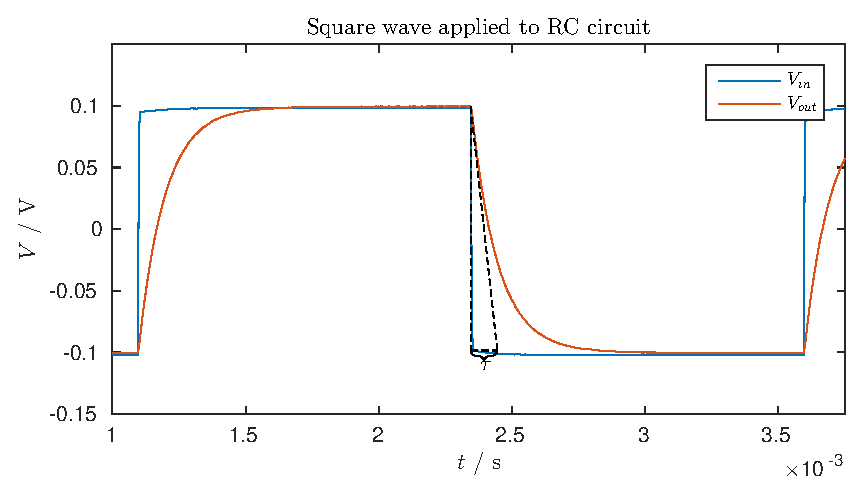
\includegraphics{ex1-step.eps}
    \caption{Square wave input to the RC circuit and the output signal. The time constant is shown for the falling edge.}
    \label{fig:ex1-1}
\end{figure}
\begin{figure}[!htb]
    \center
    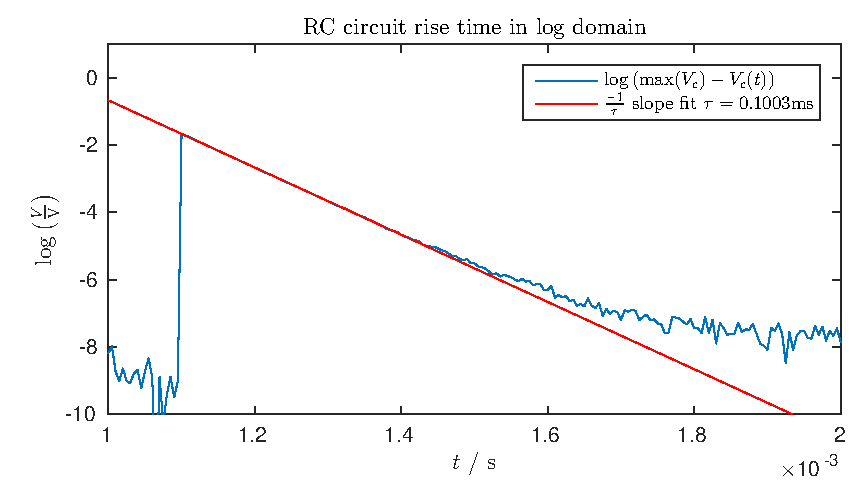
\includegraphics{ex1-log.eps}
    \caption{The difference between the final and immediate values of the output voltage during a discharge with a line fit to find \(\tau\).}
    \label{fig:ex1-2}
\end{figure}
\section{The RC Integrator}
We built an RC circuit using a 22 kOhm resistor and 47 nF capacitor which theoretically yields a time constant of
\begin{equation*}
    \tau = RC = 0.1034 \mathrm{ms}
\end{equation*}
Fig.~\ref{fig:ex1-1} shows the input and outputs of the circuit when a 100 mV PP square wave with a frequency of 1 kHz is applied at the input around
a DC bias voltage of 2 V. We find the actual time constant of the circuit by fitting a line to the difference between the 
final output value and the immediate value as seen in Fig.~\ref{fig:ex1-2}. 

We find a time constant of 0.1003 ms which is well within the tolerance of the components used to construct the circuit.
\begin{figure}[!htb]
    \center
    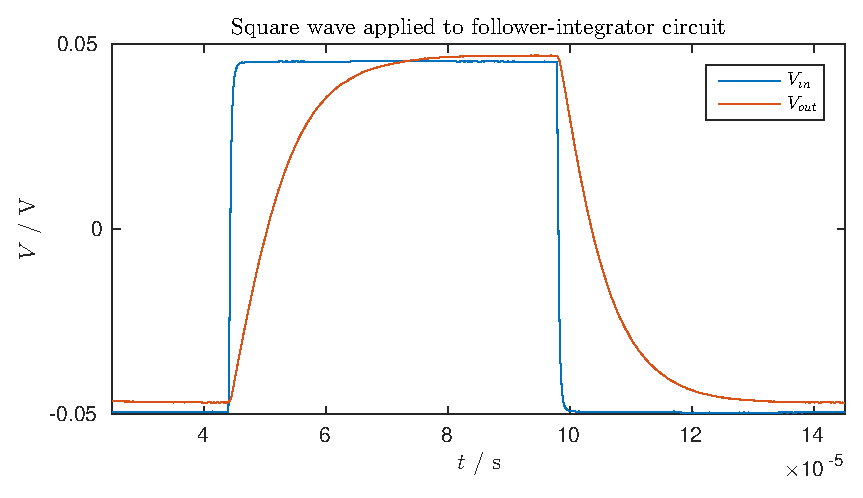
\includegraphics{ex2-step.eps}
    \caption{Square wave input to the RC circuit and the output signal. The output reaches a higher voltage than the input square wave
    because of the non-zero offset voltage for 0 output current.}
    \label{fig:ex2-1}
\end{figure}
\begin{figure}[!htb]
    \center
    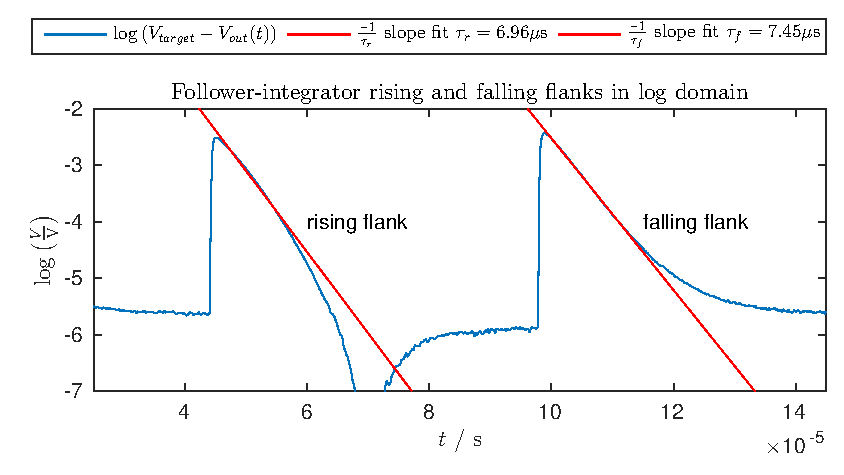
\includegraphics{ex2-log.eps}
    \caption{The difference between the final and immediate values of the output voltage during charge and discharge of the output capacitor. 
    Lines are fit to the rising and falling edges to find \(\tau_r\) and \(\tau_f\) respectively.}
    \label{fig:ex2-2}
\end{figure}
\section{Time-Domain Response of Follower-Integrator}
Fig.~\ref{fig:ex2-1} shows the output of the follow-integrator when the input is driven by a 50 mV PP square wave with a frequency of 5 kHz biased around
2 VDC. Fig.~\ref{fig:ex2-2} shows the log of the difference between the target voltage for the output and the immediate value.
The falling and rise edge time constants are found by fitting lines to these curves.

We find that the rising time constant is smaller than the falling one, therefore the circuit can more quickly respond to a 
positive differential input voltage, which indicates that the zero-current offset voltage of the transconductance amplifier is
negative. We find that the rising time and falling time constants, respectively, are
\begin{equation*}
    \tau_r = 6.96\mu\mathrm{s} \; \tau_f = 7.45\mu\mathrm{s}
\end{equation*}

The mean of the output is higher than the mean of the output because of the non-zero offset voltage in the transconductance amplifier
which results in a zero output current. The difference between the signal means is equal to this offset.

\section{Frequency-Domain Response of the Follower-Integrator}
\begin{figure}
    \center
    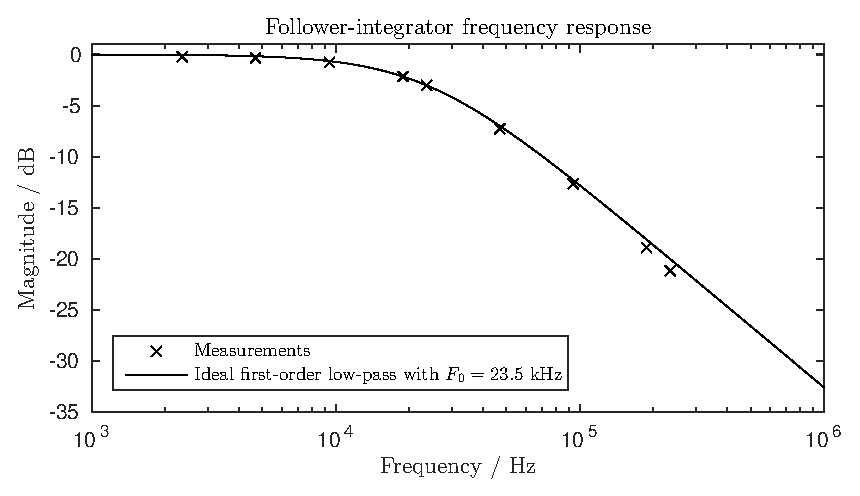
\includegraphics{ex3-freqresp.eps}
    \caption{Frequency response of the follower integrator and a theoretical ideal first-order low-pass filter. The cutoff frequency is 23.5 kHz.}
    \label{fig:ex3-1}
\end{figure}
Fig.~\ref{fig:ex3-1} shows our measurements of the frequency response for the follower-integrator. We first honed in on the cutoff frequency manually
and after this took logarithmically spaced measurements of the input-output magnitude. The line is the frequency response for a first order low-pass
filter with a cutoff frequency of 23.5 kHz. The measurements drop off more quickly, indicating some second order capacitive effects in the circuit,
stemming from parasitic capacitances and inductances in the breadbord and connecting wires.

A cutoff frequency of 23.5 kHz, implies that the time constant of the circuit is
\begin{equation*}
    \tau = \frac{1}{2\pi F_0} = 6.77 \mu\mathrm{s}
\end{equation*}
Which is slightly below the value obtained in experiment 2. However, in experiment 2, the frequency was 5 kHz, while the cutoff frequency here is 23.5 kHz which
may influence the rise and fall times for a non-ideal circuit.

\section{Large Signal Behaviour of the Follower-Integrator}
\subsection{Slew-Rate Limiting}
\begin{figure}
    \center
    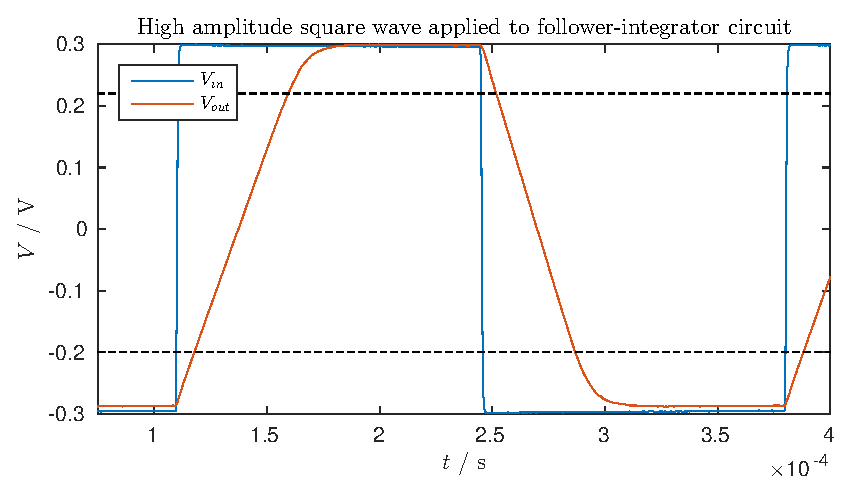
\includegraphics{ex4-slew.eps}
    \caption{Large signal input-output relation in the time domain for the follower-integrator. The dotted lines represent the limits of up and downgoing slew-rate limited operation.}
    \label{fig:ex4-1}
\end{figure}
Fig.~\ref{fig:ex4-1} shows a large signal square wave applied to the follower integrator. With this input, the circuit is slew-rate limited
and the charging of the capacitor proceeds linearly until the differential voltage is a small signal again.

The slew-rate time constants for the upgoing and downgoing edges are
\begin{equation*}
    \tau_r = 97.90\mu\mathrm{s} \; \tau_f = 83.03\mu\mathrm{s}
\end{equation*}
And their ratio 
\begin{equation*}
    \frac{\tau_r}{\tau_f} = 1.18
\end{equation*}
The difference is caused by the same effect as the offset voltage discussed earlier, the mismatch of the input transistors and current mirror transistors.
Because of the non-zero offset, a positive differential input will in this case result in a smaller magnitude of positive output current, than the corresponding
magnitude of negative output current when the differential input is negative.
\subsection{DC level manipulation}
We fixed the bias transistor voltage to 0.75 V and observed the circuit as we changed the DC level of the input from 2 V to 0.25 V in steps. Figs.~\ref{fig:ex4-2} through
\ref{fig:ex4-4} show the time-domain relationship between the input and output voltages measured at the transconductance amplifier terminals for several input bias voltages.
\begin{figure}[!htb]
    \center
    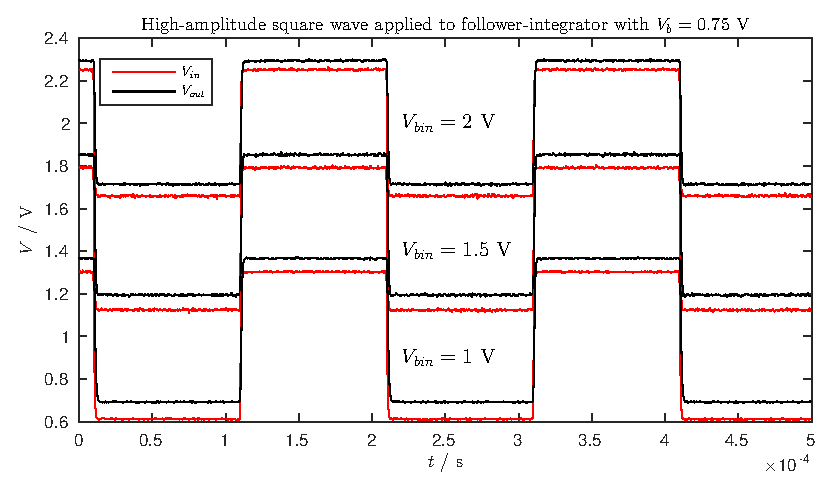
\includegraphics{ex4-1.eps}
    \caption{Input-output relationship in the time domain for a square wave input to the follower-integrator circuit with different input DC offsets.}
    \label{fig:ex4-2}
\end{figure}
\begin{figure}[!htb]
    \center
    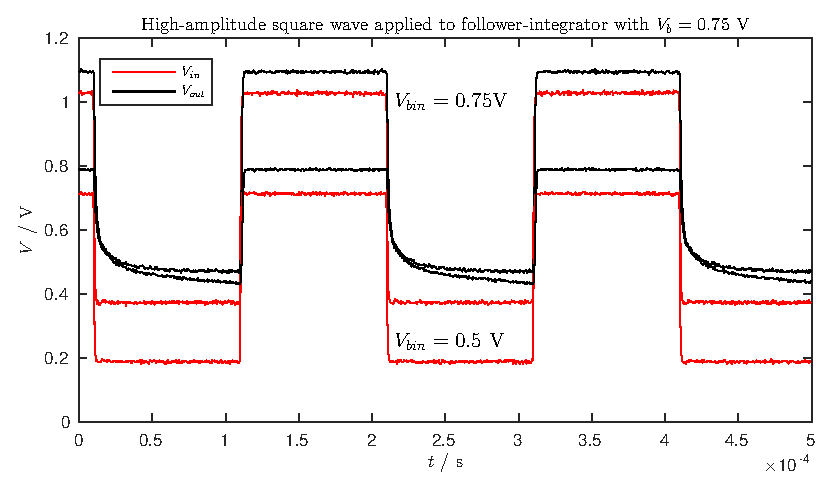
\includegraphics{ex4-2.eps}
    \caption{Input-output relationship in the time domain for a square wave input to the follower-integrator circuit with different input DC offsets. Here the
    input transistors go into the ohmic region on the downgoing flank.}
    \label{fig:ex4-3}
\end{figure}
\begin{figure}[!htb]
    \center
    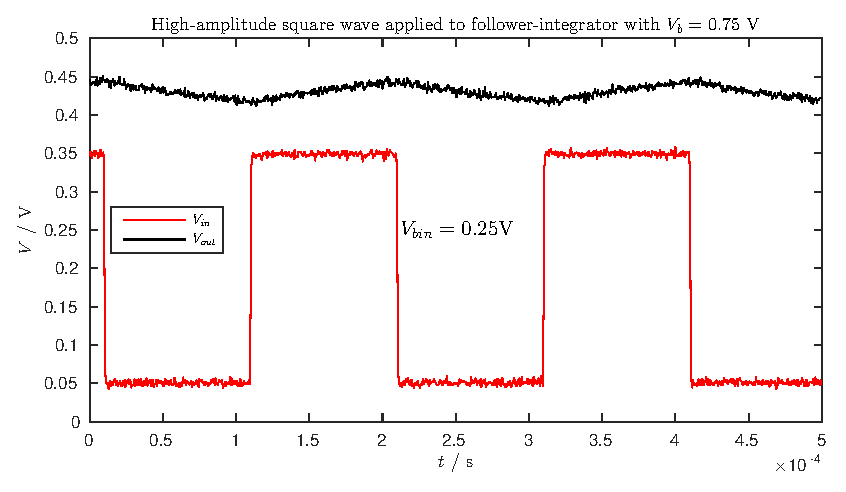
\includegraphics{ex4-3.eps}
    \caption{Input-output relationship in the time domain for a square wave input to the follower-integrator circuit for a very low DC offset which puts both
    input transistors in the ohmic region.}
    \label{fig:ex4-4}
\end{figure}
Initially, in Fig.~\ref{fig:ex4-2}, the output still faithfully follows the input because the input transistors are still operating in saturation. However the 
amplitude of the input and output signals go up because the input impedance changes.

In Fig.~\ref{fig:ex4-3} the input bias voltage is at a point where the differential input voltage holds one transistor in saturation and one in the triode region.
Resulting in the circuit being able to follow the upgoing edges, but not the downgoing ones because the current through the output transistors become very small
with the small drive.

Fig.~\ref{fig:ex4-4} shows the result of biasing both input transistors in the triode region and applying a signal that does not cause either of them to enter
saturation. The output current is now a triangle wave because of the constant current charging and discharging the capacitor.

\section{How Slow can You Integrate?}
\begin{figure}
    \center
    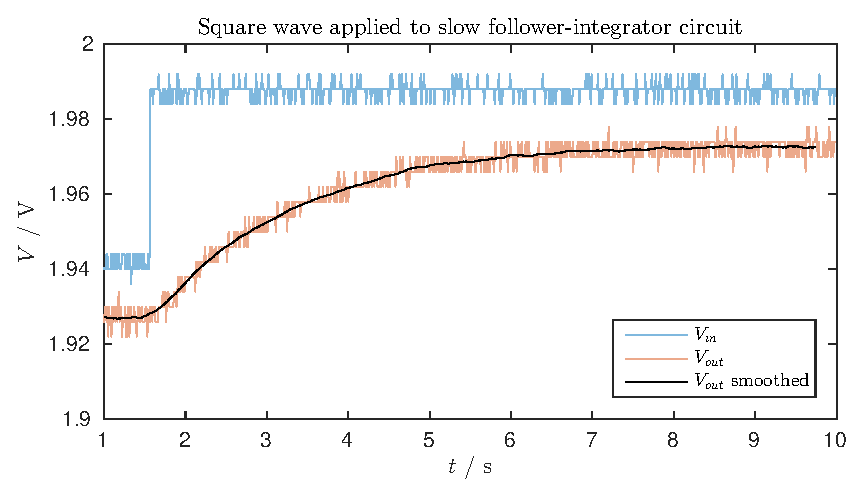
\includegraphics{ex5-step.eps}
    \caption{Square wave input to the slow follower-integrator circuit and the output signal. The output signal is smoothed using a 50-sample delay adjusted moving
    average filter to clearly show the exponential voltage increase.}
    \label{fig:ex5-1}
\end{figure}
\begin{figure}
    \center
    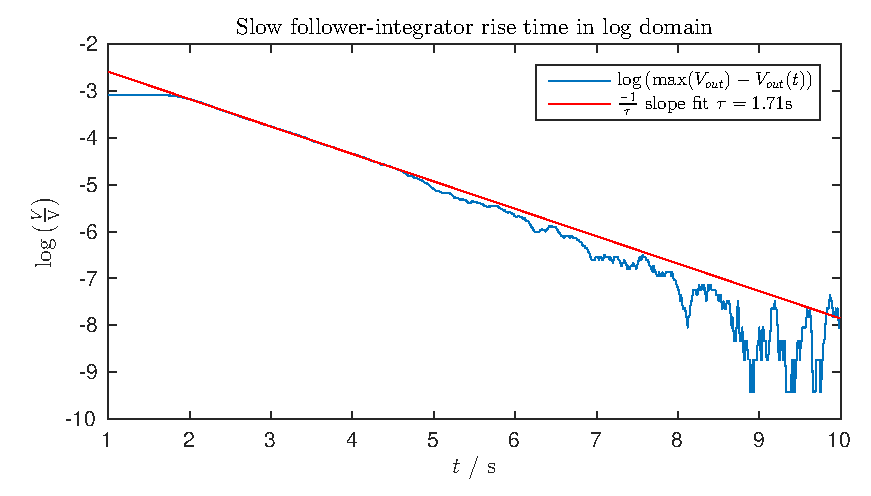
\includegraphics{ex5-log.eps}
    \caption{The difference between the final and immediate values of the output voltage during a charge cycle with a line fit to find \(\tau = 1.7\)s.}
    \label{fig:ex5-2}
\end{figure}
Fig.~\ref{fig:ex5-1} shows the time-domain response of the transconductance amplifier follower-integrator circuit with a bias voltage of 0 V read from the multimeter
connected to the potbox, and an input bias of 2 V DC. The input is a 50 mV PP square wave. Fig.~\ref{fig:ex5-2} shows the difference between the final value of the
output and the immediate value. From this, the time constant of the circuit is found to be
\begin{equation*}
    \tau = 1.7 \mathrm{s}
\end{equation*}
When the follower-integrator circuit is made very slow, the offset moves from being positive to negative, relative to the applied square wave. It also
drops with the DC voltage.
\end{document}
